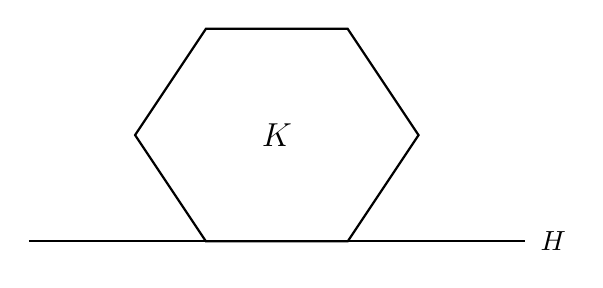
\begin{tikzpicture}[thick, scale=0.9]

    % 1. 绘制水平直线 H
    \draw (-1, 0) -- (6, 0) node[right=2pt] {$H$};

    % 2. 绘制上方的多边形（凸集 K），底边与直线 H 重合
    \draw (1.5, 0) -- (3.5, 0) -- (4.5, 1.5) -- (3.5, 3) -- (1.5, 3) -- (0.5, 1.5) -- cycle; % cycle 用于闭合路径

    % 3. 在多边形中心添加标签 K
    \node at (2.5, 1.5) {\large $K$};

\end{tikzpicture}